\documentclass[12pt]{article}
\usepackage[english]{babel}
\usepackage[utf8]{inputenc}

%% Pointer to 'default' preamble, other reusable files
% pacakages and definitions

\usepackage{geometry}
\geometry{
	letterpaper, 
	portrait, 
	top=.75in,
	left=.8in,
	right=.75in,
	bottom=.5in		} 	% Page Margins
	
%% additional packages for nice things
\usepackage{amsmath} 	% for most math
\usepackage{commath} 	% for abs
\usepackage{lastpage}	% for page count
\usepackage{amssymb} 	% for therefore
\usepackage{graphicx} 	% for image handling
\usepackage{wrapfig} 	% wrap figures
\usepackage[none]{hyphenat} % for no hyphenations
\usepackage{array} 		% for >{} column characterisctis
\usepackage{physics} 	% for easier derivative \dv....
\usepackage{tikz} 		% for graphic@!
\usepackage{circuitikz} % for circuits!
\usetikzlibrary{arrows.meta} % for loads
\usepackage[thicklines]{cancel}	% for cancels
\usepackage{xcolor}		% for color cancels
\usepackage[per-mode=fraction]{siunitx} % for si units and num
\sisetup{group-separator = {,}, group-minimum-digits = 3} % additional si unit table functionality

\usepackage{fancyhdr} 	% for header
\usepackage{comment}	% for ability to comment out large sections
\usepackage{multicol}	% for multiple columns using multicols
\usepackage[framed,numbered]{matlab-prettifier} % matlab sytle listing
\usepackage{marvosym} 	% for boltsymbol lightning
\usepackage{pdflscape} 	% for various landscape pages in portrait docs.
%\usepackage{float}
\usepackage{fancyvrb}	% for Verbatim (a tab respecting verbatim)
\usepackage{enumitem}	% for [resume] functionality of enumerate
\usepackage{spreadtab} 	% for using formulas in tables}
\usepackage{numprint}	% for number format in spread tab
\usepackage{subcaption} % for subfigures with captions
\usepackage[normalem]{ulem} % for strike through sout

% for row colors in tables....
\usepackage{color, colortbl}
\definecolor{G1}{gray}{0.9}
\definecolor{G2}{rgb}{1,0.88,1}%{gray}{0.6}
\definecolor{G3}{rgb}{0.88,1,1}

% For table formatting
\usepackage{booktabs}
\renewcommand{\arraystretch}{1.2}
\usepackage{floatrow}
\floatsetup[table]{capposition=top} % put table captions on top of tables

% Caption formating footnotesize ~ 10 pt in a 12 pt document
\usepackage[font={small}]{caption}

%% package config 
\sisetup{output-exponent-marker=\ensuremath{\mathrm{E}}} % for engineer E
\renewcommand{\CancelColor}{\color{red}}	% for color cancels
\lstset{aboveskip=2pt,belowskip=2pt} % for more compact table
%\arraycolsep=1.4pt\def
\setlength{\parindent}{0cm} % Remove indentation from paragraphs
\setlength{\columnsep}{0.5cm}
\lstset{
	style      = Matlab-editor,
	basicstyle = \ttfamily\footnotesize, % if you want to use Courier - not really used?
}
\renewcommand*{\pd}[3][]{\ensuremath{\dfrac{\partial^{#1} #2}{\partial #3}}} % for larger pd fracs
\renewcommand{\real}[1]{\mathbb{R}\left\{ #1 \right\}}	% for REAL symbol
\newcommand{\imag}[1]{\mathbb{I}\left\{ #1 \right\}}	% for IMAG symbol
\definecolor{m}{rgb}{1,0,1}	% for MATLAB matching magenta
	
%% custom macros
\newcommand\numberthis{\addtocounter{equation}{1}\tag{\theequation}} % for simple \numberthis command

\newcommand{\equal}{=} % so circuitikz can have an = in the labels
\newcolumntype{L}[1]{>{\raggedright\let\newline\\\arraybackslash\hspace{0pt}}m{#1}}
\newcolumntype{C}[1]{>{\centering\let\newline\\\arraybackslash\hspace{0pt}}m{#1}}
\newcolumntype{R}[1]{>{\raggedleft\let\newline\\\arraybackslash\hspace{0pt}}m{#1}}

%% Header
\pagestyle{fancy} % for header stuffs
\fancyhf{}
% spacing
\headheight 29 pt
\headsep 6 pt
%%% custom commands for nicer units
\newcommand{\mw}{\ensuremath{\text{ MW}}}
\newcommand{\hz}{\ensuremath{\text{ Hz}}}
\newcommand{\pu}{\ensuremath{\text{ Pu}}}
\newcommand{\sbase}{\ensuremath{\text{S}_{\text{Base}}}}
\newcommand{\fbase}{\ensuremath{f_{\text{Base}}}}
\newcommand{\mbase}[1]{\ensuremath{\text{M}_{\text{Base}_{#1}}}}
\newcommand{\hsys}{\ensuremath{\text{ H}_{\text{sys}}}}


%% Header
\rhead{Thad Haines \\ Page \thepage\ of \pageref{LastPage}}
\chead{Talking Points \\ Week of June 24th, 2019}
\lhead{Research \\ }

\begin{document}
\begin{multicols}{2}
\raggedright
	\paragraph{Recent Progress:}
	\begin{enumerate}

		\item \textbf{PSLF License Expires June 30}.

		\item $R_{eff}$ removed from simulation.

		\item Multiple Generators per bus tested as working.

		\item First Balancing Authority Agent tested on six machine system.

		\item Timer and Power Plant Agents added.

	%	\item More \verb|matplotlib| plot functions created.

		\item GitHub updated:\\
		\verb|https://github.com/thadhaines/|
		
	\end{enumerate}
\paragraph{Current Tasks:}
	\begin{enumerate}

		\item Continue to Update Code flowchart to aid in further development.

		\item Work to incorporate Matt's \emph{Suggested Use Cases} into simulation.
		\begin{itemize}
		
		\item Add Shunt Group Agent
		\item Work to Define Definite Time Controller user input
		
		\item Refine Agent actions for \\ AGC/LFC (i.e. ACE / UCE / SCE calculations)
		\item Test Generator and line tripping events.

		\end{itemize}
		%\item Keep Goals and Requests in mind.
		
		%\subitem A FlowtabrDAO exists that can find flow between busses. A way to initialize bus connections between areas has yet to be devised.

	\end{enumerate}
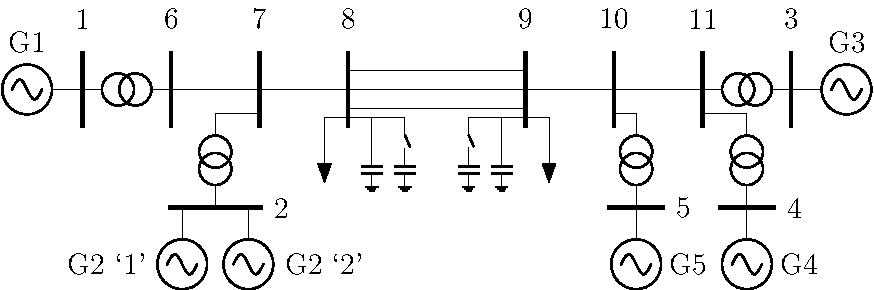
\includegraphics[width=\linewidth]{../../models/sixMachine/sixMachine}
\vfill\null
\columnbreak
	\paragraph{Current Questions:}
	\begin{enumerate}

	\item What should be included in BA options? (Filtering, Distribution options...)
	\item How to handle non governed Machines on AGC? (ramp Pm?)
	
	%	\item Overview of planned PSLF scenarios? $\rightarrow$ Similar to Heredia paper but on Wecc/MiniWecc Scale? 
		
	%	\item Is there more available/relevant event data that may help us to verify simulations of specific instances (wind ramps or other behavior) that novel research will focus on? %(Heredia paper data helpful for some wind ramp data context)

	%	\item  Any progress / continued interest in miniWecc Area definitions?



%\pagebreak


\paragraph{Future Tasks:} %(Little to No Progress since last time / Things coming down the pipe)
	\begin{enumerate}

		\item Formulate feasible plan of action for casting all WECC governors to LTD governors (tgov1). Something like:
		\begin{enumerate}
		\item Parse models of interest from dyd.
		\item Create dyd from parsed model.
		\item Automate a 'scaled' Pref step test for a one machine infinite bus in PSDS.
		\item Read and analyze output data
		\item Generate/Calculate LTD equivalent model parameters from results (this will probably use MATLAB and \verb|jfind|)
		\item Export custom dyd for LTD simulation. (PSDS would still use original the dyd, though \emph{could} use modified dyd)
		\end{enumerate}

		\item Add import mirror / bypass mirror init sequence option to prevent repeated mirror creations.

		\item Create an agent for every object: \\ ULTC, SVD, Transformer, \ldots
		
		\item Investigate line current data and ULTC action in PSDS.
		
		\item Account for different types of loads (exponential load model)
	\end{enumerate}

\paragraph{Matt Requests:}
\begin{enumerate}
		\item Enable multiple dyd files to overwrite / replace previously defined agents/parameters
		\item Allow for variable time steps.
\end{enumerate}

	\end{enumerate}

%\paragraph{'Soft Goals':}
%	\begin{enumerate}
%	\item Simulate 10$\times$ faster than PSDS.\\ Not met --- MiniWECC $\approx$8x faster.\\Varies with system size \& time step.
%	\end{enumerate}
		

\vfill\null

\end{multicols}

\pagebreak
\paragraph{Initial BA Results:} A 75 MW step in load took place in Area 2. Since Area 2 was already importing $\approx$100 MW, the BA action increased generation in Area 2. Eventaully, ACE and Interchange Error go to zero and frequency returns to 60 Hz.
\begin{figure}[h!]
		\centering
		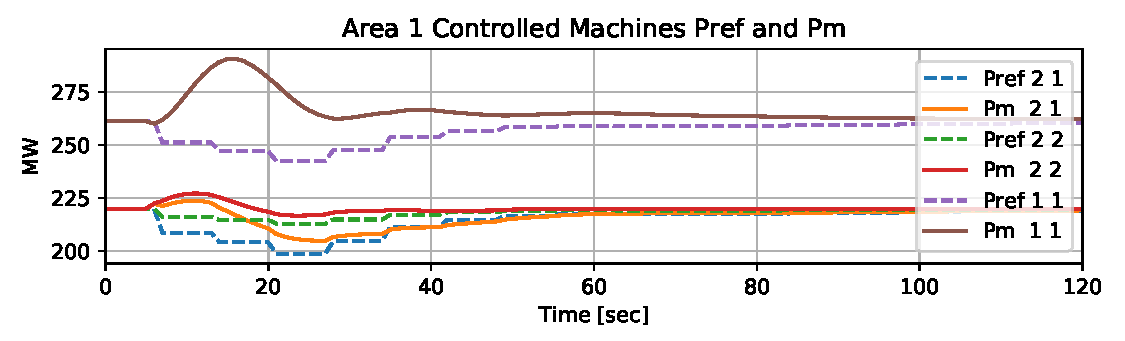
\includegraphics[width=\linewidth]{area1}\vspace{-1em}
		%\caption{Generator Electrical Power Output}
		%\label{ Pe}		 
\end{figure}\vspace{-2em}
\begin{figure}[h!]
		\centering
		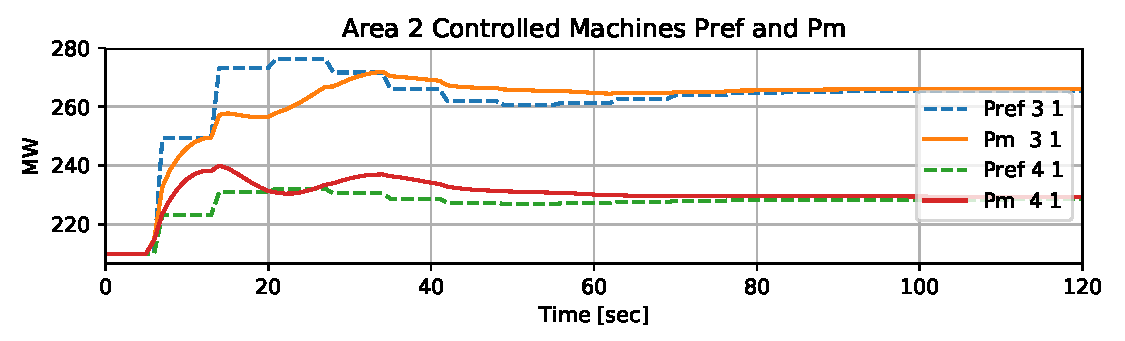
\includegraphics[width=\linewidth]{area2}\vspace{-1em}
		%\caption{Generator Mechanical Power Output (un-governed machines have no PSDS data)}
		%\label{ Pm}		 
\end{figure}\vspace{-2em}
\begin{figure}[h!]
		\centering
		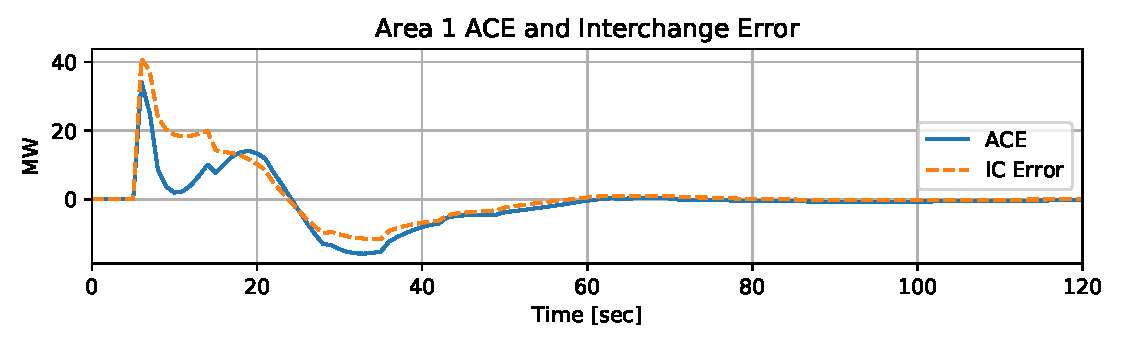
\includegraphics[width=\linewidth]{ACE}\vspace{-1em}
		%\caption{Reactive Power Output}
		%\label{ Q}		 
\end{figure}\vspace{-2em}
\begin{figure}[h!]
		\centering
		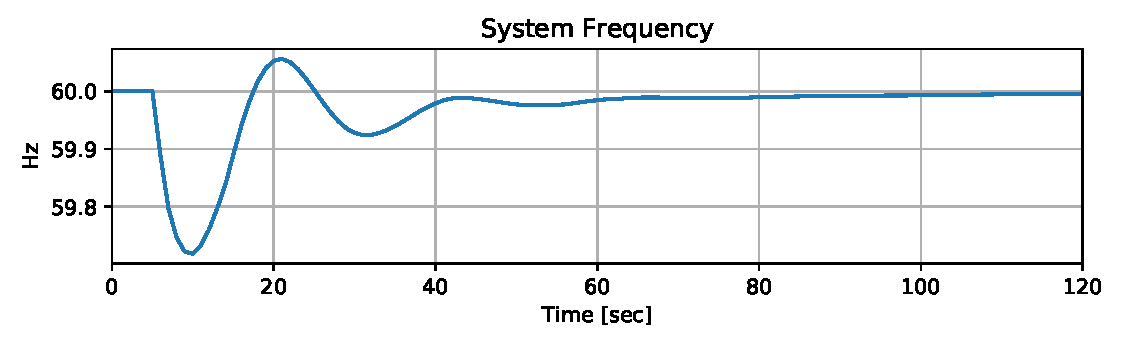
\includegraphics[width=\linewidth]{freq}\vspace{-1em}
		%\caption{Reactive Power Output}
		%\label{ Q}		 
\end{figure}\vspace{-2.5em}
\end{document}